\chapter{Background Estimation}

\section{Introduction}

The Standard Model backgrounds to the search are estimated.  

\section{Backgrounds}

QCD is the largest background. QCD events are balanced. Any missing transverse
energy comes from detector imperfections. There are three different components 
to the QCD background:

\begin{itemize}
\item {\bf Fakes from jets ($\pi^{0}\rightarrow\gamma\gamma$):} $\pi^{0}$s are
one of the main constituents of jets. The two photons from a high energy 
$\pi^{0}$ can easily be mistaken for a single photon. Most $\pi^{0}$s in jets
will be non-isolated due to the surronding HCAL energy and tracks. However
there is a distribution of isolation and given the large cross section of QCD, 
some of these events will end up in the isolated tail.
\item {\bf Prompt $\gamma$+jet:} In these events the photon comes directly from
the parton hard scattering. The other jet can come from gluon radiation or
jet fragmentation. These events contain prompt photons which tend to be isolated
and have good shower shape. The $\pT$ of the photons is distributed around half
the $\HT$ of the event.
\item {\bf QCD jets with ISR/FSR:} A QCD jets event where an initial state quark
or final state quark radiates a photon. These events also contain prompt photons
which tend to be isolated and have good shower shape. The cross section of this 
process falls with the $\pT$ of the photon. 
\end{itemize}

The Electroweak background is small in comparison to the QCD background.
Electroweak processes can contribute real $\MET$ by the neutrino which is not
detected by CMS. The cross section of electroweak processes is much lower than
that of QCD and this rules out any background due to fakes from jets. There are
two possible sources of photons: $W\rightarrow e\nu$ where the electron has been
misidentied as a photon or $\gamma Z\rightarrow\gamma\nu\nu$ which has a real
photon. \\

The $t\bar{t}$ background has real photons and real $\MET$, but it is negligible 
due to the low cross section. The $t\bar{t}$ background is estimated using Monte
Carlo. The W/Z+$\gamma$ cross section is also negligible due to the high HT
requirement.

\section{QCD Background}
\label{sec:QCD_Background}

All three sources of QCD background have fake $\MET$ due to detector effects.
Fake $\MET$ can come from the HCAL resolution or from severe mismeasurements
such as dead ECAL Trigger Towers or poor HCAL response. \\

ECAL Trigger Towers are $5\times5$ arrays of crystals in the ECAL with the
photodetectors behind them and the electronics to trigger and read out the data. 
There are $82\times72$ trigger towers in the ECAL barrel. Some of these Trigger
Towers are dead i.e. there is no data coming from them. This means that any
objects going down a dead Trigger Tower will be missed causing fake $\MET$. The 
number of dead Trigger Towers may vary from run to run as those with a problem 
are masked and those which have been fixed are unmasked. Some ECAL Trigger 
Towers have long-term problems. There are about XX dead ECAL TTs: YY of these 
have trigger information available. Figure \ref{fig:Dead_ECAL_TTs} shows a map 
of ECAL Trigger Towers. \\

Poor HCAL response is another cause of large fake $\MET$. Sometimes a jet is
reconstructed with a much lower $\pT$ than it actually has. Such mismeasurements
are extremely pathelogical and not at all well understood. These are not
correlated with any specific region of the detector. \\

The core resolution is approximately Gaussian in x and y components of $\MET$ 
while the severe mismeasurements contribute a non-Gaussian tail to the $\MET$ 
distribution. Both components scale up with $\HT$. The core resolution scales as
$\sim\sqrt{\HT}$ while the tails increase because higher $\HT$ events contain 
higher $\pT$ objects which give larger $\MET$ when missed. \\

Any background estimation method needs to be able to estimate these detector 
effects. If the Monte Carlo were to be used we would be relying on its ability 
to correctly model all the causes of fake $\MET$. Not just the core resolution 
but also the $\MET$ tail with severe mismeasurements. Using a control sample 
from data gives a perfect simulation of the CMS detector. The problem is reduced
to finding a control sample with the same kinematic properties as the selected 
sample rather than trying to simulate the most extreme elements of detector
response. \\

A control sample is defined to contain events which pass all the selection 
criteria except for the isolation. This control sample is used to estimate the
$\MET$ shape of the QCD background in each $\HT$ bin. The absolute number of
events is obtained by normalising the $\MET$ distribution to the number of
events with $\MET < 50 \GeV$. \\

The assumption in this method is that the control sample has the same $\MET$
distribution as the selected sample in each $\HT$ bin. The control sample is
very similar to the selected sample. It has the same objects with the same
kinematic cuts. All events contain at least one photon with good shower shape.
The only difference is that in the control sample the photon is non-isolated
while in the selected sample it happens to be isolated. Although they contain
the three sources of QCD background in different proportions, in both cases the 
source of $\MET$ is the same: detector effects. So we can expect them to have 
the same $\MET$ distributions. \\

The background estimation is shown to work in Monte Carlo and in data using a 
sideband region. Figure \ref{fig:Regions} shows the regions used for the
background estimation. The (non-isolated) control sample is used to estimate the 
background in the (isolated) selected sample. The sideband region is used to
check that the background estimation works i.e. the non-isolated and isolated 
samples have the same $\MET$ distribution. \\

\begin{figure}
\begin{center}
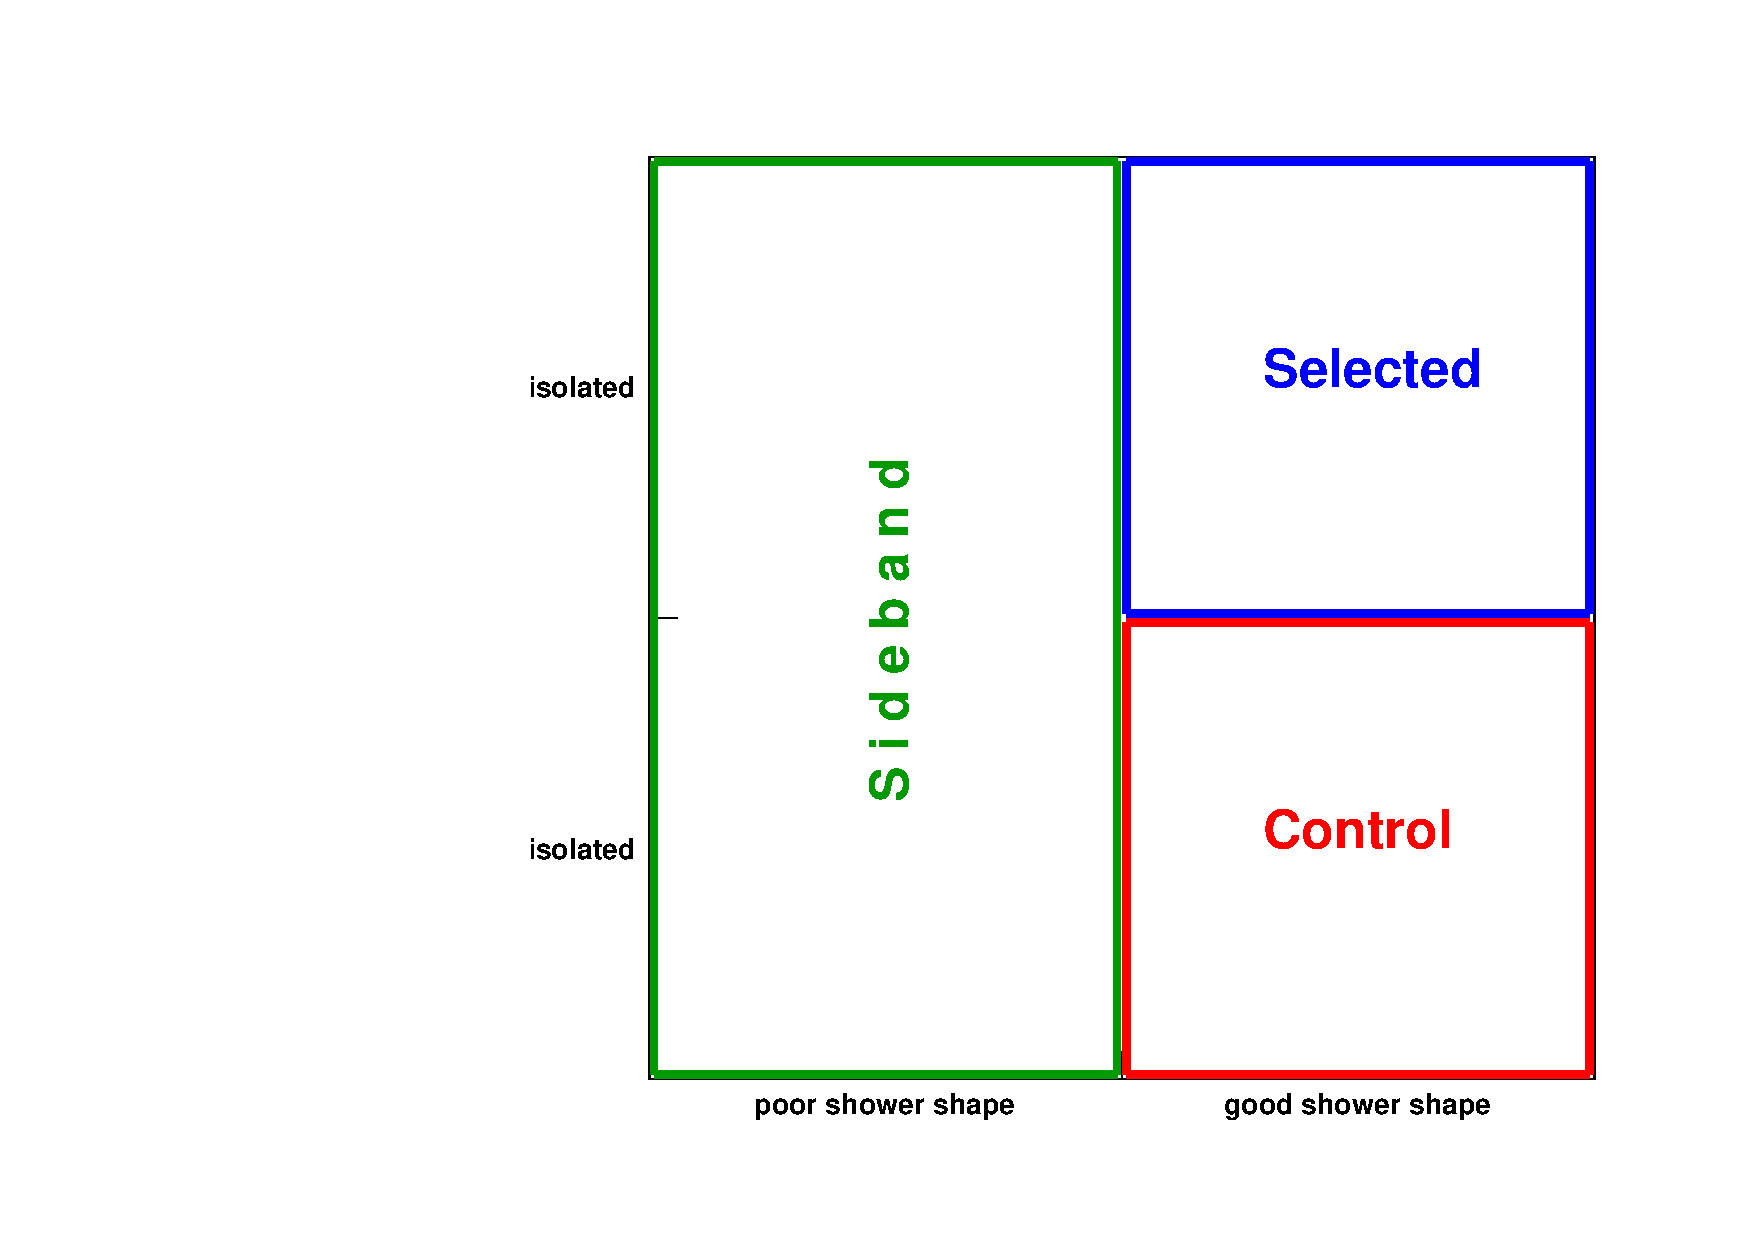
\includegraphics[width=0.8\textwidth]{Regions.pdf}
\end{center}
\caption{A graphic showing the layout of the regions used for the QCD background
estimation. The control sample is used to estimate the $\MET$ distribution in
the selected sample. The sideband region is used to check that the background
estimation works.}
\label{fig:Regions}
\end{figure}

Figure \ref{fig:Bkgd_Est_MC} shows the background estimation and the number of
selected events in bins of $\HT$ and $\MET$ for the Monte Carlo. \\

\begin{figure}
\includegraphics[width=0.5\textwidth]{mc_QCD.pdf}
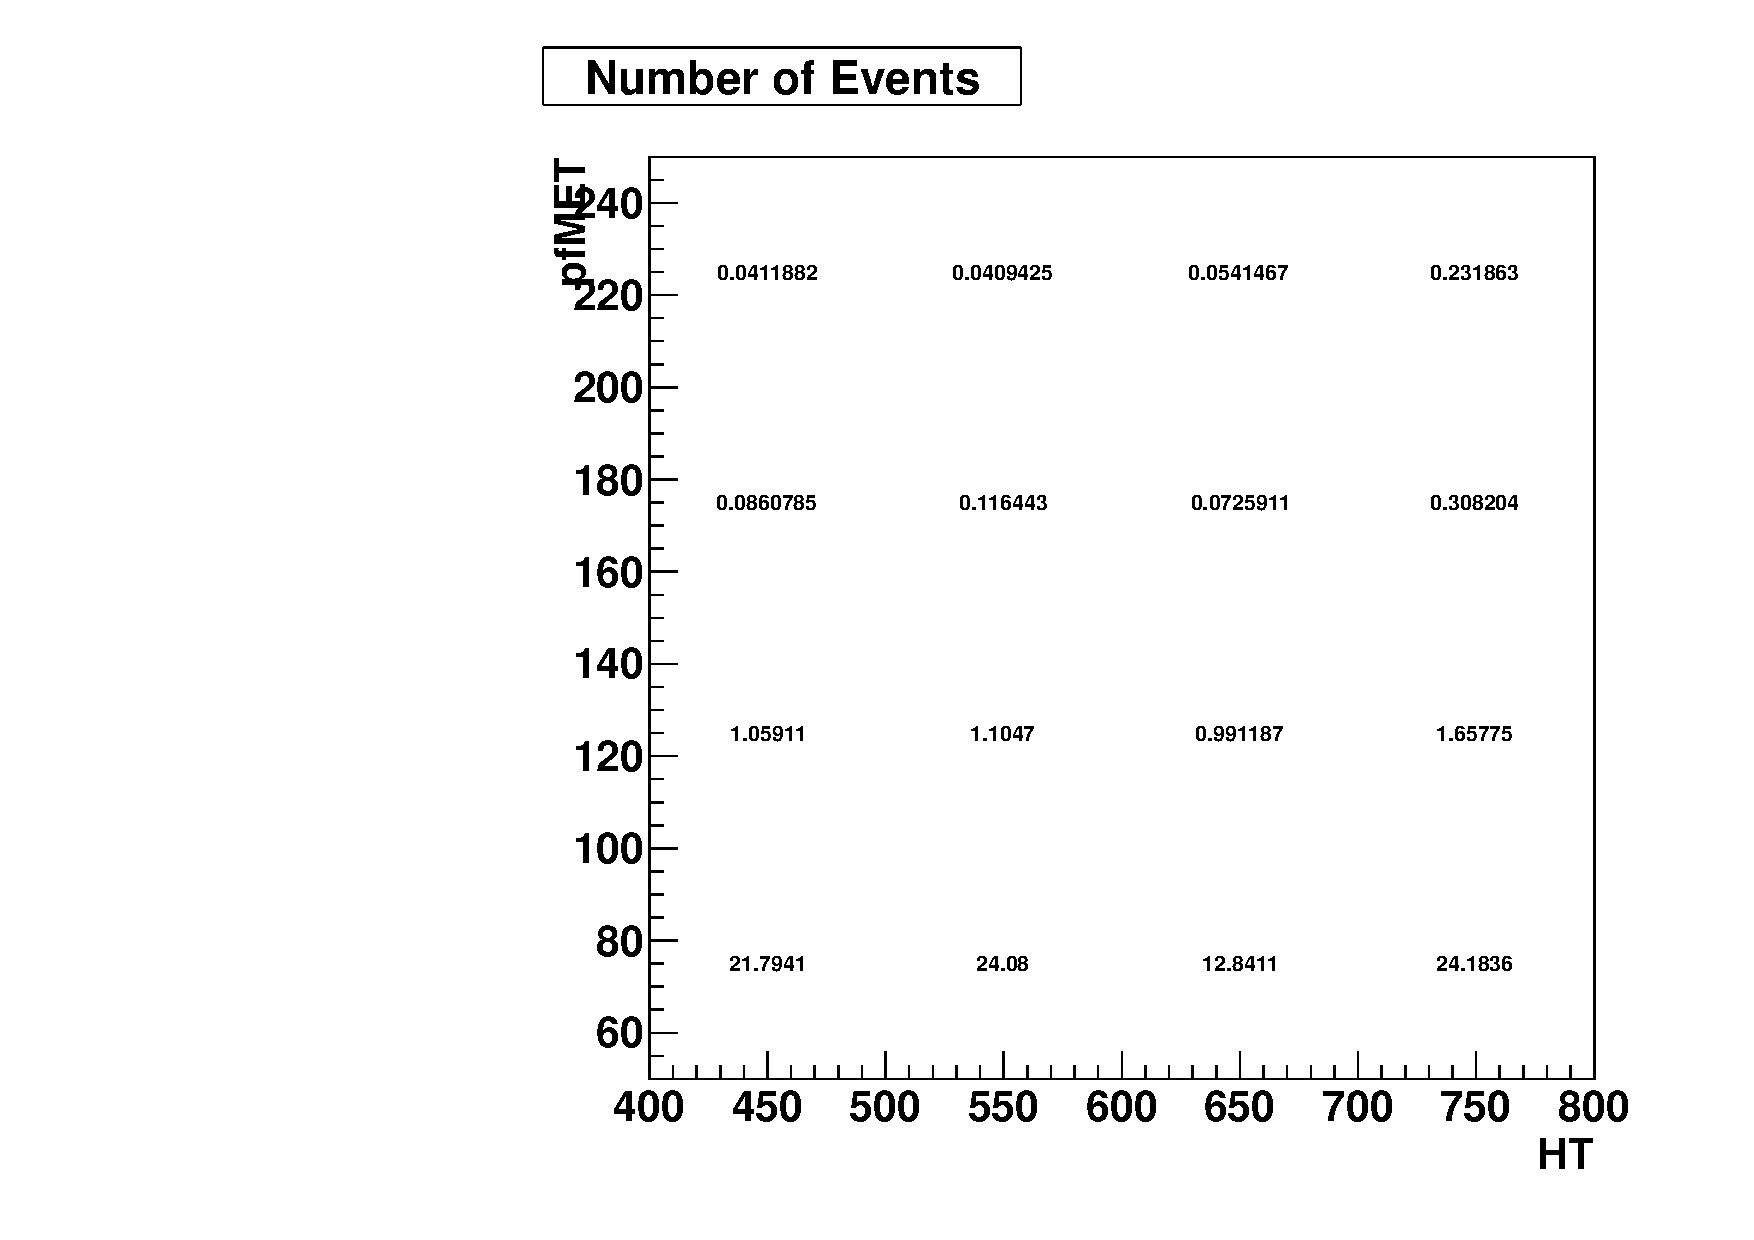
\includegraphics[width=0.5\textwidth]{mc_Data.pdf}
\caption{The background estimation (left) and number of selected events (right) 
in bins of $\HT$ and $\MET$ in the Monte Carlo to check that the background
estimation method works.}
\label{fig:Bkgd_Est_MC}
\end{figure}

Figure \ref{fig:Bkgd_Est_Sideband} shows the estimation of the number of
isolated events in bins of $\HT$ and $\MET$ using the non-isolated sample in the
sideband region from data compared to the true number of events. \\

\begin{figure}
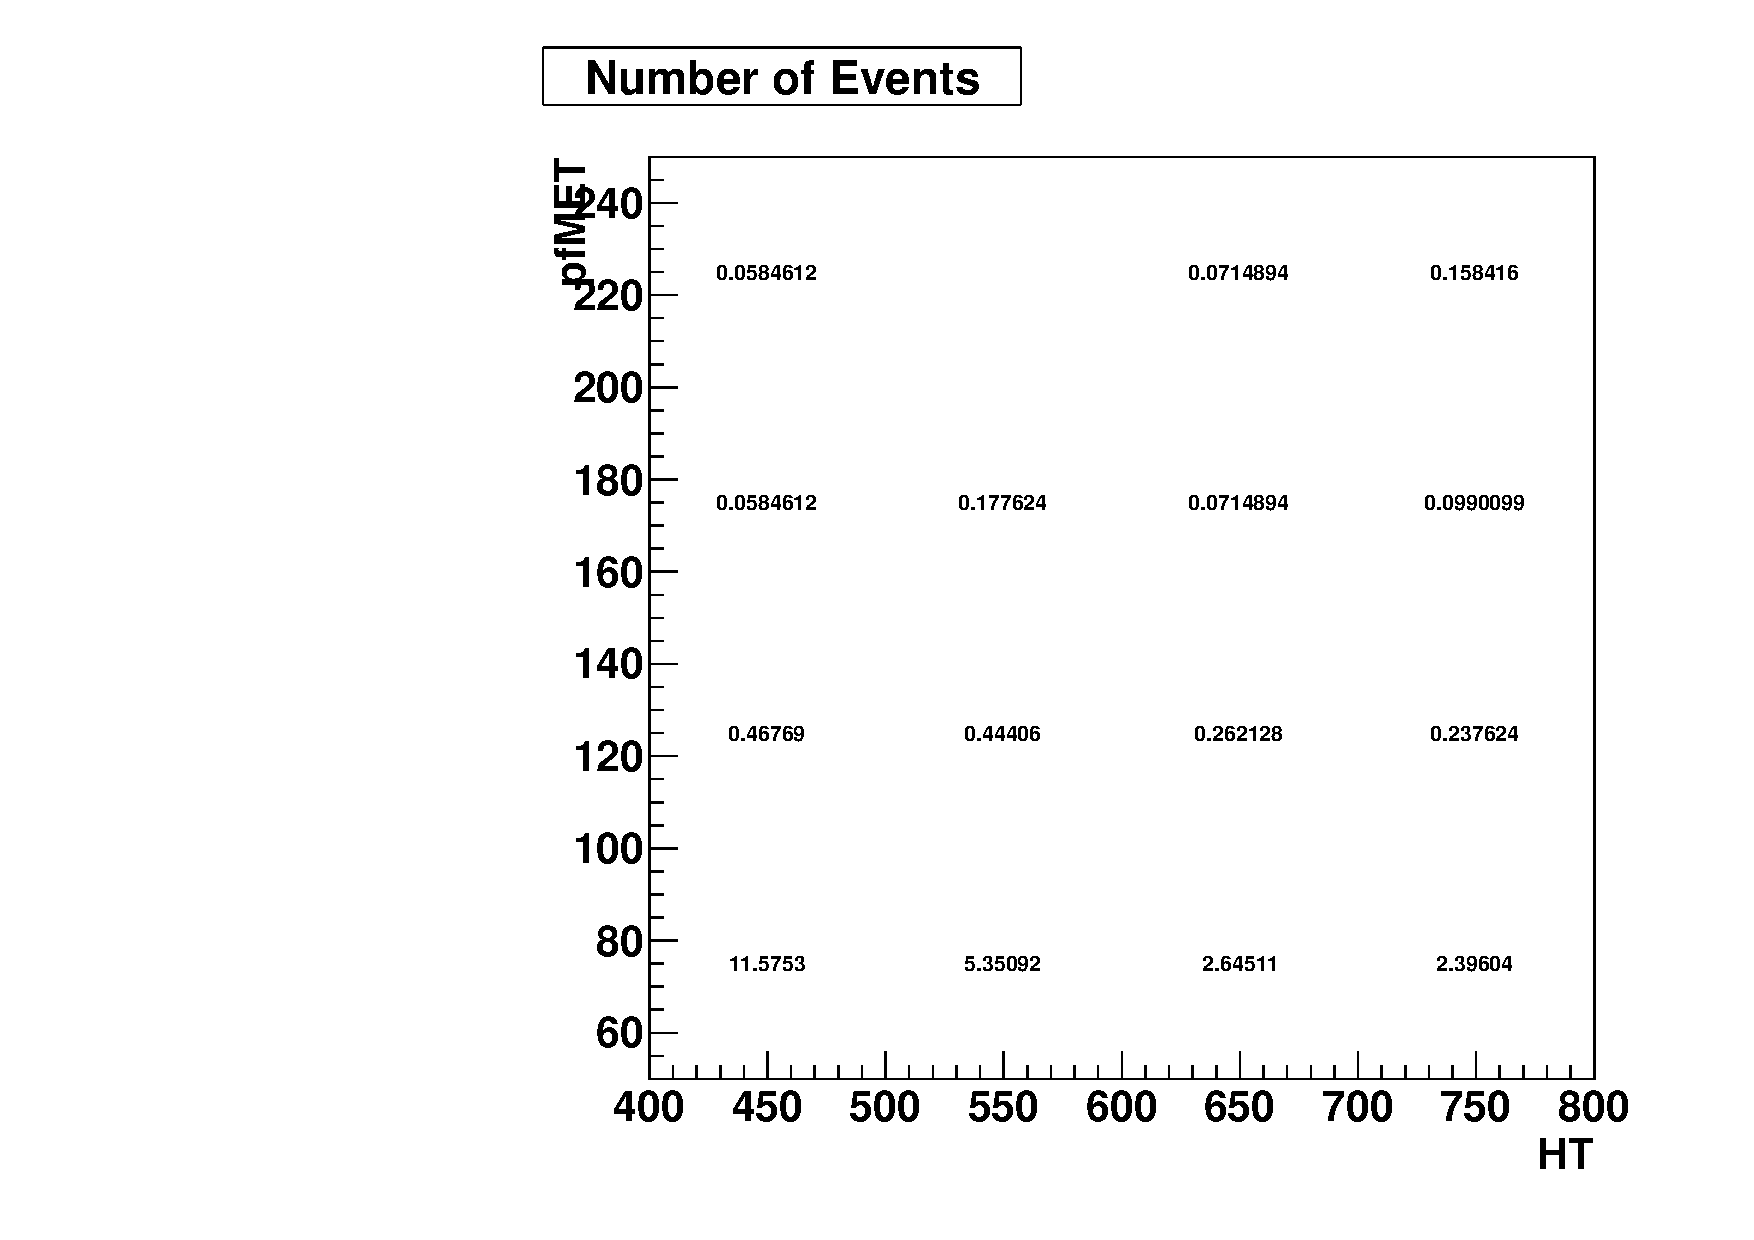
\includegraphics[width=0.5\textwidth]{sb_QCD.pdf}
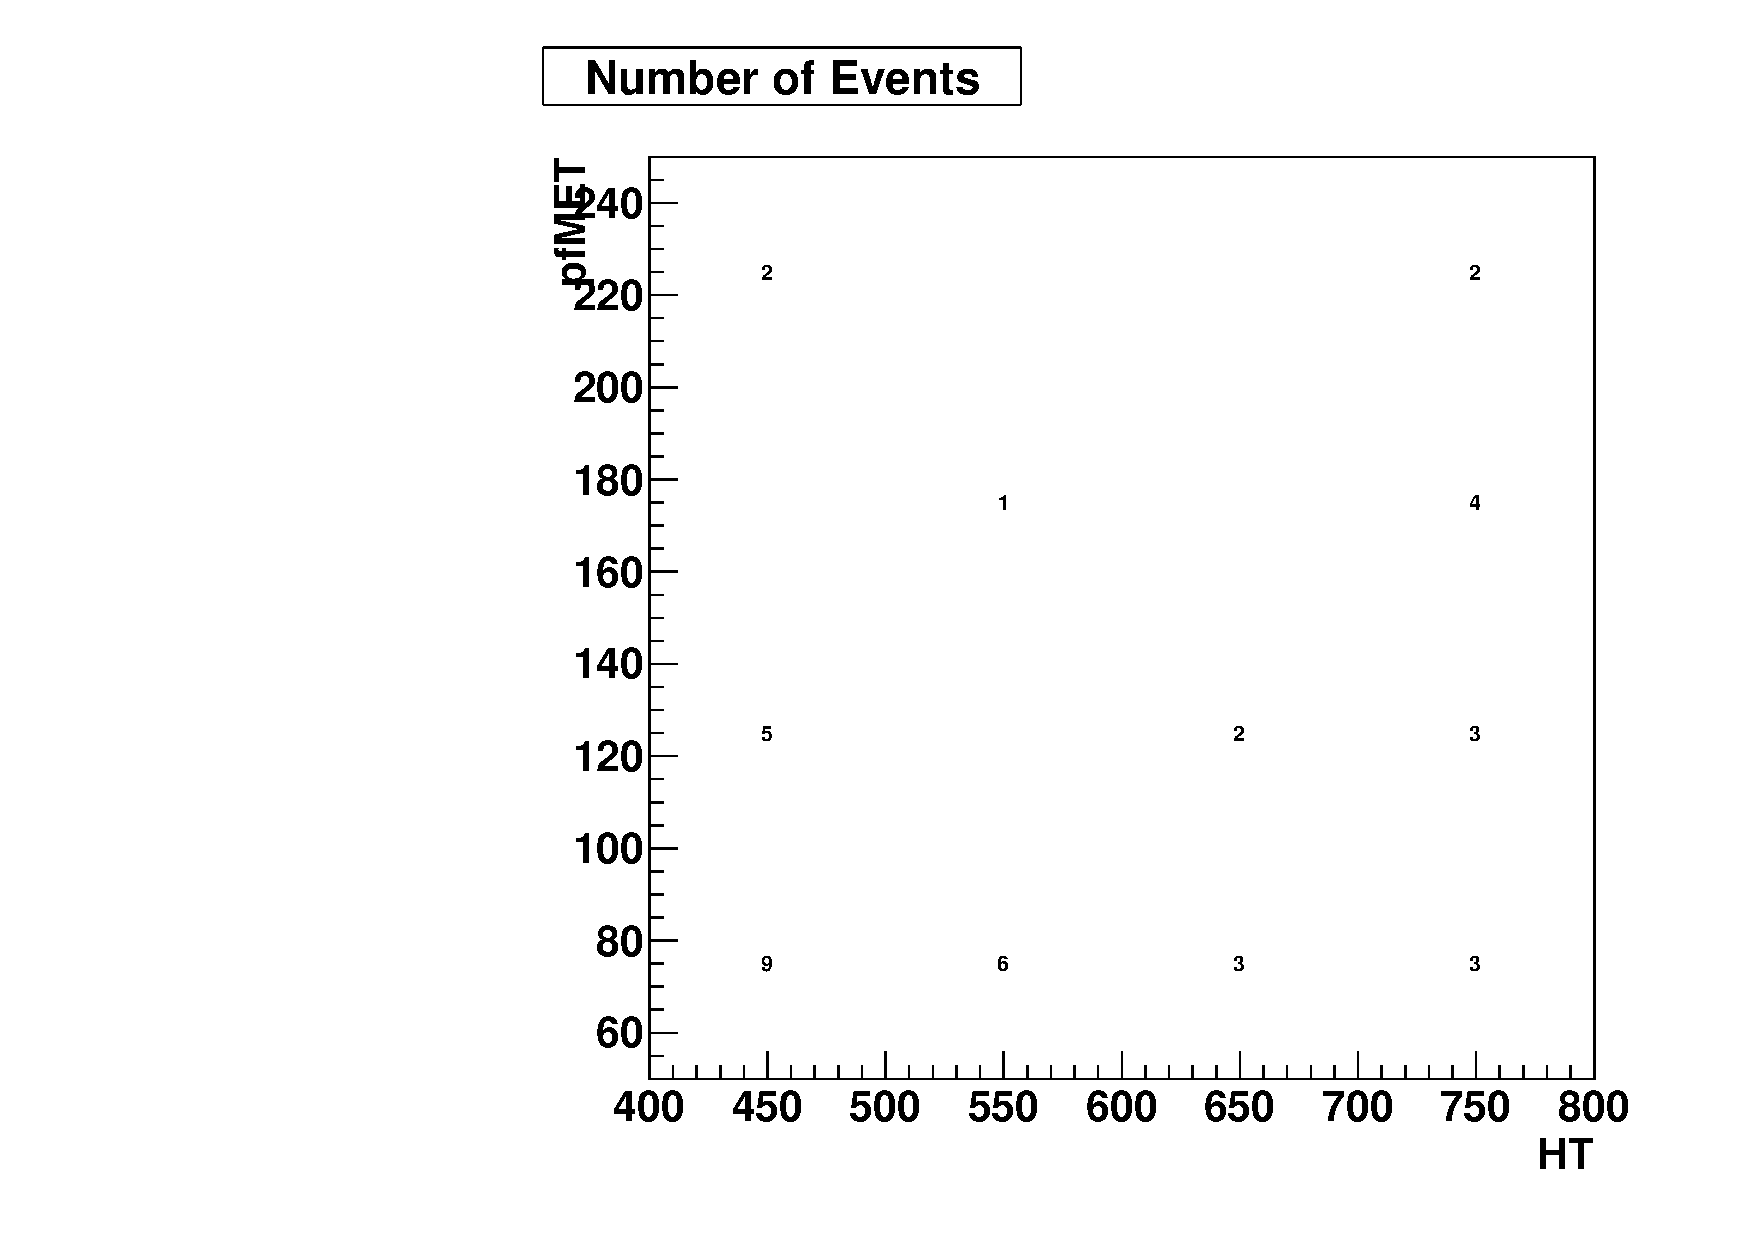
\includegraphics[width=0.5\textwidth]{sb_Data.pdf}
\caption{The estimation of the number of isolated events (left) using the
non-isolated events in the sideband region from data compared to the true number
(right).}
\label{fig:Bkgd_Est_Sideband}
\end{figure}

A systematic error on the assumption is taken as half the difference between the
estimated number of events and true number of events in Monte Carlo.

\section{Electroweak Background}

Electroweak processes can have real MET due to neutrinos which are not
detected by CMS. There are two components to the electroweak background:
$W\rightarrow e\nu$, where the electron is misidentified as a photon and 
$\gamma Z\rightarrow\gamma\nu\nu$, which has a real photon and real MET. \\

The $W\rightarrow e\nu$ background is estimated by measuring the electron/photon
misidentification rate in data. \\

The $\gamma Z\rightarrow\gamma\nu\nu$ background is estimated from Monte Carlo.

\section{Electron/Photon Fake Rate}

Measuring the fraction of electrons that are misidentified as photons is
important for estimating the background coming from $W\rightarrow e\nu$ events
where the electron is misidentified as a photon. \\

With a fake rate, $f_{e\rightarrow\gamma}$, and given a true number of
$Z\rightarrow ee$ events, $N_{Z}$, the number of events in the ee sample is
given by $N_{ee} = (1 - f_{e\rightarrow\gamma})^{2}N_{Z}$. And the number of
events in the e$\gamma$ is given by $N_{e\gamma} = 2[f_{e\rightarrow\gamma}(1 -
f_{e\rightarrow\gamma})]N_{Z}$. With measurements of $N_{ee}$ and $N_{e\gamma}$
the fake rate can be determined as $f_{e\rightarrow\gamma} =
N_{e\gamma}/(2N_{ee} + N_{e\gamma})$. \\

The fake rate is measured using an ee sample and an e$\gamma$ sample from data.
Electrons are selected using the same requirements as photons, but with a pixel
seed required (rather than no pixel seed). The number of $Z\rightarrow ee$
events in each sample is determined by fitting a Crystal Ball function with a
linear background assumption (Figure \ref{fig:Zee_Fit}). There is no significant
difference in the yields if a constsnt or quadratic background shape is used. \\

\begin{figure}
\begin{center}
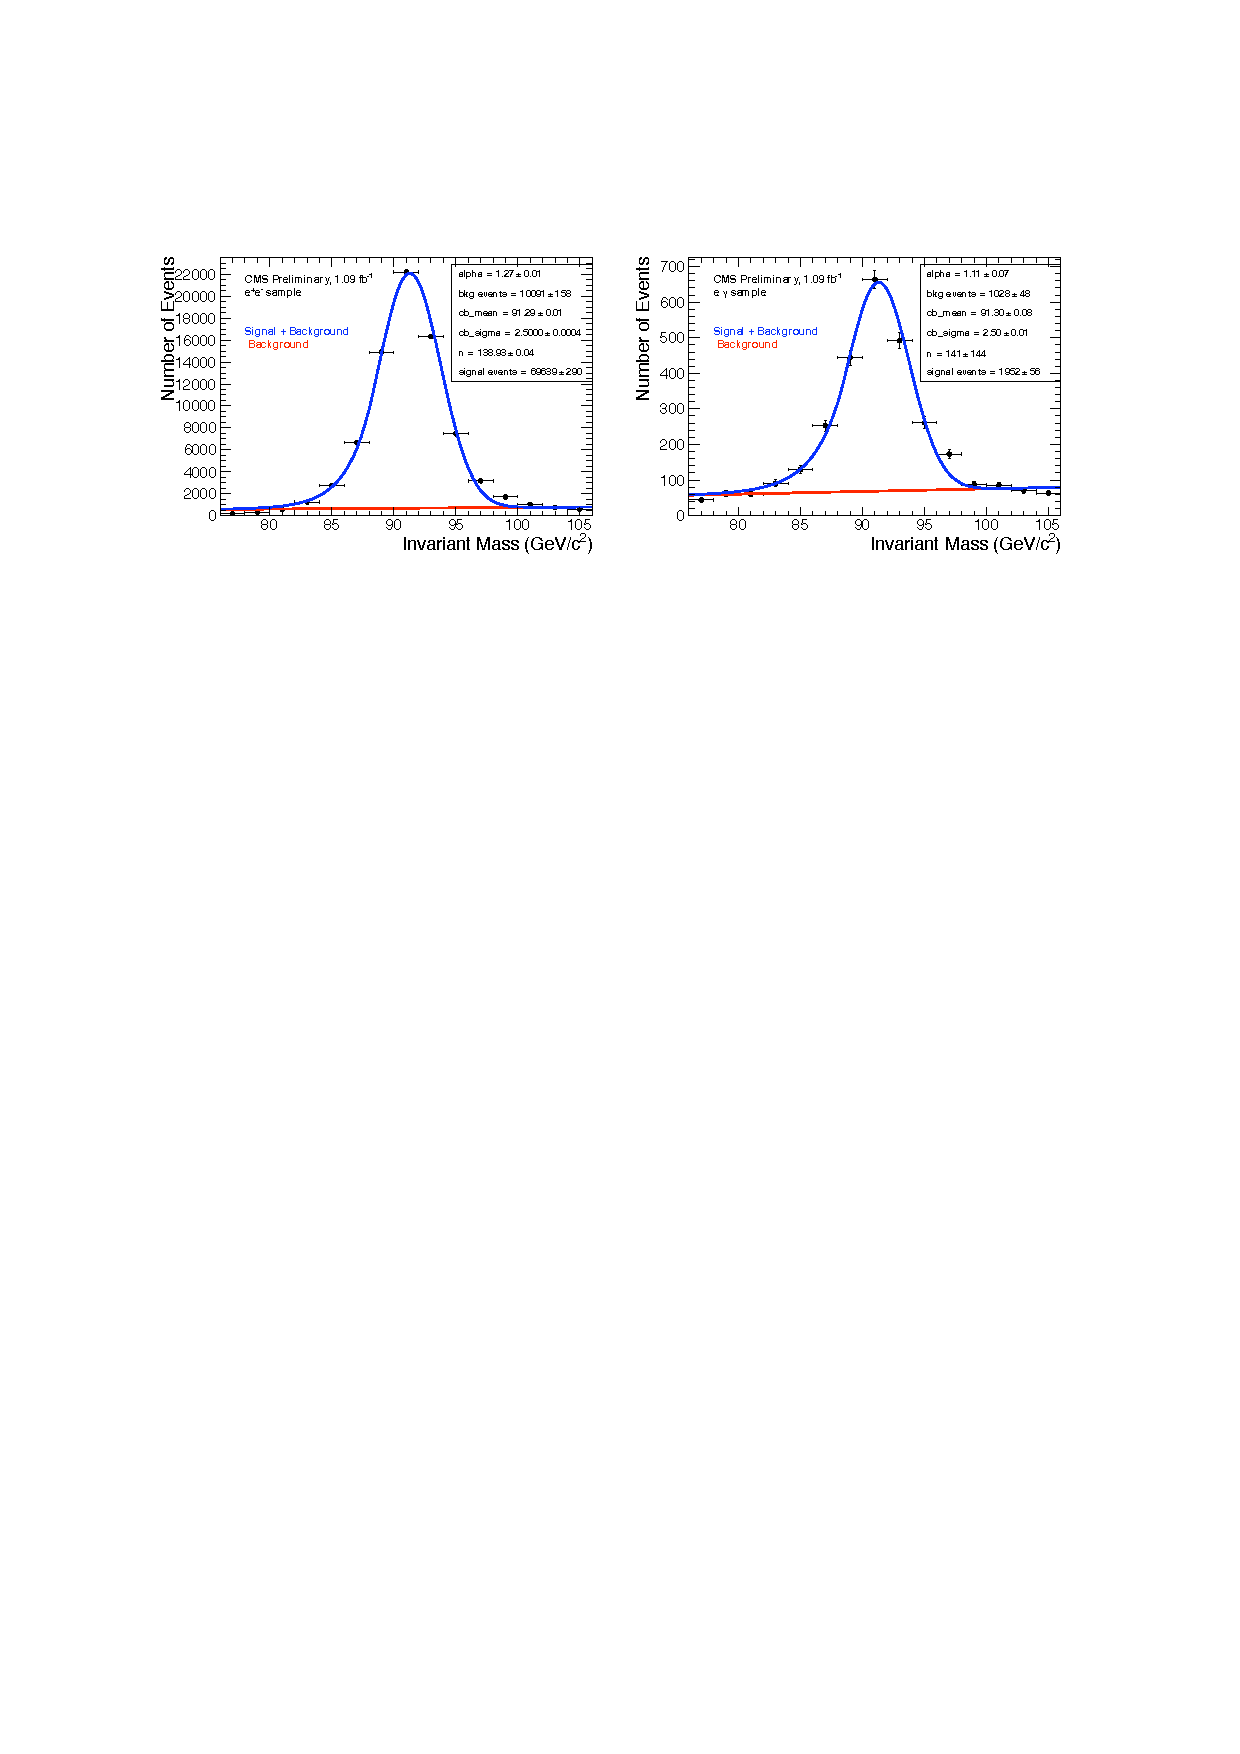
\includegraphics[width=1.0\textwidth]{Zee_Fit.pdf}
\end{center}
\caption{The invariant mass of ee and e$\gamma$ candidates. The Z peak is fitted
using a Crystal Ball function and a linear background.}
\label{fig:Zee_Fit}
\end{figure}

The fit of the Z peak in the ee sample yields $69639 \pm 290$ Z events. Fitting
the Z peak in the e$\gamma$ sample yield $1952\pm56$ Z events. From these
numbers the misidentification rate is $f_{e\rightarrow\gamma} = 0.014\pm0.004$.
This number varies little as a function of e or $\gamma$ $p_{T}$. Based on the
variations with $p_{T}$ a systematic uncertainty of 0.002 is assigned to
$f_{e\rightarrow\gamma}$. 

\section{Conclusions}
